\PassOptionsToPackage{unicode=true}{hyperref} % options for packages loaded elsewhere
\PassOptionsToPackage{hyphens}{url}
%
\documentclass[]{article}
\usepackage{lmodern}
\usepackage{amssymb,amsmath}
\usepackage{ifxetex,ifluatex}
\usepackage{fixltx2e} % provides \textsubscript
\ifnum 0\ifxetex 1\fi\ifluatex 1\fi=0 % if pdftex
  \usepackage[T1]{fontenc}
  \usepackage[utf8]{inputenc}
  \usepackage{textcomp} % provides euro and other symbols
\else % if luatex or xelatex
  \usepackage{unicode-math}
  \defaultfontfeatures{Ligatures=TeX,Scale=MatchLowercase}
\fi
% use upquote if available, for straight quotes in verbatim environments
\IfFileExists{upquote.sty}{\usepackage{upquote}}{}
% use microtype if available
\IfFileExists{microtype.sty}{%
\usepackage[]{microtype}
\UseMicrotypeSet[protrusion]{basicmath} % disable protrusion for tt fonts
}{}
\IfFileExists{parskip.sty}{%
\usepackage{parskip}
}{% else
\setlength{\parindent}{0pt}
\setlength{\parskip}{6pt plus 2pt minus 1pt}
}
\usepackage{hyperref}
\hypersetup{
            pdfborder={0 0 0},
            breaklinks=true}
\urlstyle{same}  % don't use monospace font for urls
\usepackage[margin=1in]{geometry}
\usepackage{graphicx,grffile}
\makeatletter
\def\maxwidth{\ifdim\Gin@nat@width>\linewidth\linewidth\else\Gin@nat@width\fi}
\def\maxheight{\ifdim\Gin@nat@height>\textheight\textheight\else\Gin@nat@height\fi}
\makeatother
% Scale images if necessary, so that they will not overflow the page
% margins by default, and it is still possible to overwrite the defaults
% using explicit options in \includegraphics[width, height, ...]{}
\setkeys{Gin}{width=\maxwidth,height=\maxheight,keepaspectratio}
\setlength{\emergencystretch}{3em}  % prevent overfull lines
\providecommand{\tightlist}{%
  \setlength{\itemsep}{0pt}\setlength{\parskip}{0pt}}
\setcounter{secnumdepth}{0}
% Redefines (sub)paragraphs to behave more like sections
\ifx\paragraph\undefined\else
\let\oldparagraph\paragraph
\renewcommand{\paragraph}[1]{\oldparagraph{#1}\mbox{}}
\fi
\ifx\subparagraph\undefined\else
\let\oldsubparagraph\subparagraph
\renewcommand{\subparagraph}[1]{\oldsubparagraph{#1}\mbox{}}
\fi

% set default figure placement to htbp
\makeatletter
\def\fps@figure{htbp}
\makeatother


\author{}
\date{\vspace{-2.5em}}

\begin{document}

National Coral Reef Monitoring Program

Climate Monitoring Brief: Dry Tortugas National Park

\begin{center}\rule{0.5\linewidth}{0.5pt}\end{center}

\begin{figure}

{\centering \includegraphics[width=0.75\linewidth]{Data/STRfish} 

}

\caption{New Subsurface Temperature Recorder depolyed at White Shoal in Dry Tortugas National Park}\label{fig:front}
\end{figure}

Atlantic Oceanographic \& Meteorological Laboratory Coral Program
University of Miami Cooperative Institute of Marine and Atmospheric
Science National Oceanic Atmospheric Administration

N. Besemer, A. Palacio, M. Jankulak, G. Kolodziej, I. Enochs - July 2021

\begin{flushleft}\includegraphics[width=0.2\linewidth]{DRTO_Field-Report_AP_V2_files/figure-latex/logos-1} \end{flushleft}

\begin{center}\rule{0.5\linewidth}{0.5pt}\end{center}

\hypertarget{about-this-summary-brief}{%
\subsubsection{About this summary
brief}\label{about-this-summary-brief}}

The NOAA Atlantic Oceanographic and Meteorological Laboratory (AOML)
conducts the long-term National Coral Reef Monitoring Program (NCRMP) to
track the status and trends of coral reef ecosystems of the U.S.
Atlantic and Caribbean coral reef jurisdictions. This FY21 summary brief
provides an overview of the most recent survey efforts.

\hypertarget{expedition-summary}{%
\subsubsection{Expedition summary}\label{expedition-summary}}

\begin{itemize}
\tightlist
\item
  The most recent NCRMP Atlantic climate monitoring took place at Dry
  Tortugas National Park from June 24th to June 29th 2021
\item
  Four different sites were visited by 5 team members completing a total
  of 63 dives.
\item
  These sites represent temporal‐resolution monitoring with moored
  instruments at fixed time‐series which are placed on depth gradient to
  assess how vertical structure affects reef status and trends.
\end{itemize}

\begin{center}\rule{0.5\linewidth}{0.5pt}\end{center}

\hypertarget{data-collection}{%
\subsubsection{Data collection}\label{data-collection}}

\begin{itemize}
\tightlist
\item
  Subsurface \textbf{temperature} recorders (STRs) were recovered at all
  4 study sites, accounting for 1.1 million temperature observations:

  \begin{itemize}
  \tightlist
  \item
    Pulaski Shoal (1m): 311,609 observations
  \item
    White Shoal (5m): 311,213 observations
  \item
    Bird Key Reef (15m): 311,560 observations
  \item
    Black Coral Rock (25m): 165,695 observations
  \end{itemize}
\item
  At the Bird Key Reef, short term instruments (72h) were deployed to
  monitor daily fluctuations in:

  \begin{itemize}
  \tightlist
  \item
    \textbf{Current}: 880 observations
  \item
    \textbf{pH}: 879 observations
  \item
    \textbf{Light}: 876 observations
  \end{itemize}
\item
  Additionally, changes in benthic cover and carbonate production were
  monitored at Bird Key Reef by recording:

  \begin{itemize}
  \tightlist
  \item
    \textbf{Bioerosion}: 5 Bioerosion Monitoring Units (BMUs),
  \item
    \textbf{Calcification}: 5 Calcification Accretions Units (CAUs)
  \item
    \textbf{Benthic cover}: 6 landscape mosaics
  \item
    \textbf{Carbonate budget surveys}: 6 BL BLA BLA
  \end{itemize}
\end{itemize}

\begin{center}\includegraphics{DRTO_Field-Report_AP_V2_files/figure-latex/makeAmap-1} \end{center}

 \textbf{Figure 1:} Map of study sites in Dry Tortugas National Park
area

\begin{center}\rule{0.5\linewidth}{0.5pt}\end{center}

\hypertarget{temperature}{%
\paragraph{Temperature}\label{temperature}}

Three years of temperature measurements were retrieved and processed
from all 4 sites (depths). Temperature was measured using SeaBird
Electronics Subsurface Temperature Recorders (STR)s that collected data
at 5-minute intervals.

\begin{center}\includegraphics{DRTO_Field-Report_AP_V2_files/figure-latex/unnamed-chunk-1-1} \end{center}

 \textbf{Figure 2:} Temperature conditions at four sites in the Dry
Tortugas representing a depth gradient: Pulaski Shoal Lighthouse (1m)
White Shoal (5m), Bird Key Reef (15m), and Black Coral Rock (25m). Data
were collected from November 2018 to June 2021, with the exception of
the 25m STR that recorded until February 7th 2020.

Temperature values were similar among the 1m, 5m and 15m depths with the
lowest temperatures recorded during February 2021 (20.8, 20.7, and 19.9
\(^\circ\)C, respectively) and the the higest temperatures during the
summer of 2019 and 2020 (31.7, 31.6, and 31.5 \(^\circ\)C,
respectively). The 25m STR detected consistent temperature
stratification at this site during the summers when it was active.
Temperatures were XX to YY \(^\circ\)C below the values at other depths.

\begin{center}\rule{0.5\linewidth}{0.5pt}\end{center}

\hypertarget{diurnal-suite-deployment}{%
\paragraph{Diurnal Suite Deployment}\label{diurnal-suite-deployment}}

At Bird Key Reef additional instruments were deployed for a 72-hour
diurnal suite that monitored pH, temperature, light and current speed.
SeaFET pH logger, Tiltmeter and EcoPAR collected measurements at
5-minute intervals.

\begin{center}\includegraphics{DRTO_Field-Report_AP_V2_files/figure-latex/Diurnal_Suite_Plot-1} \end{center}

\textbf{Figure 3:} Bird Key Reef (15m) diurnal suite monitoring from
June 25th to 28th. Top panel: pH and temperature. Bottom panel: current
speed and Photosynthetically Available Radiation (PAR). Grey blocks
denote night time throughout sequence of plot. Instruments measured
parameters every 5 minutes.

As part of the diurnal suite, discrete water samples were collected at
three-hour intervals (n=24) using Subsurface Automatic Samplers (SAS).
THIS SAMPLES WILL BE ANALIZED TO ASSESS BLA BLA BLA

MAYBE ADD A PICTURE IF THE SAS AND OR LINK TO SAS PAGE

\begin{center}\rule{0.5\linewidth}{0.5pt}\end{center}

\hypertarget{other-deliverables}{%
\paragraph{Other Deliverables}\label{other-deliverables}}

\begin{itemize}
\tightlist
\item
  \textbf{Calcification Accretion Units (CAUs)} and \textbf{Bioerosion
  Monitoring Units (BMUs)} were collected and redeployed for the next
  sampling cycle. CAUs are processed by the Pacific Climate group and
  the data will be available within a year. BMUs will be dried and
  cleaned using a hydrogen peroxide solution. These samples will be
  weighed and scanned using a Macro CT scanner and then compared to
  their pre-scans to quantify bioerosion. Data will be available in a
  year. Please reference previous datasets for more information.
\end{itemize}

\begin{figure}

{\centering 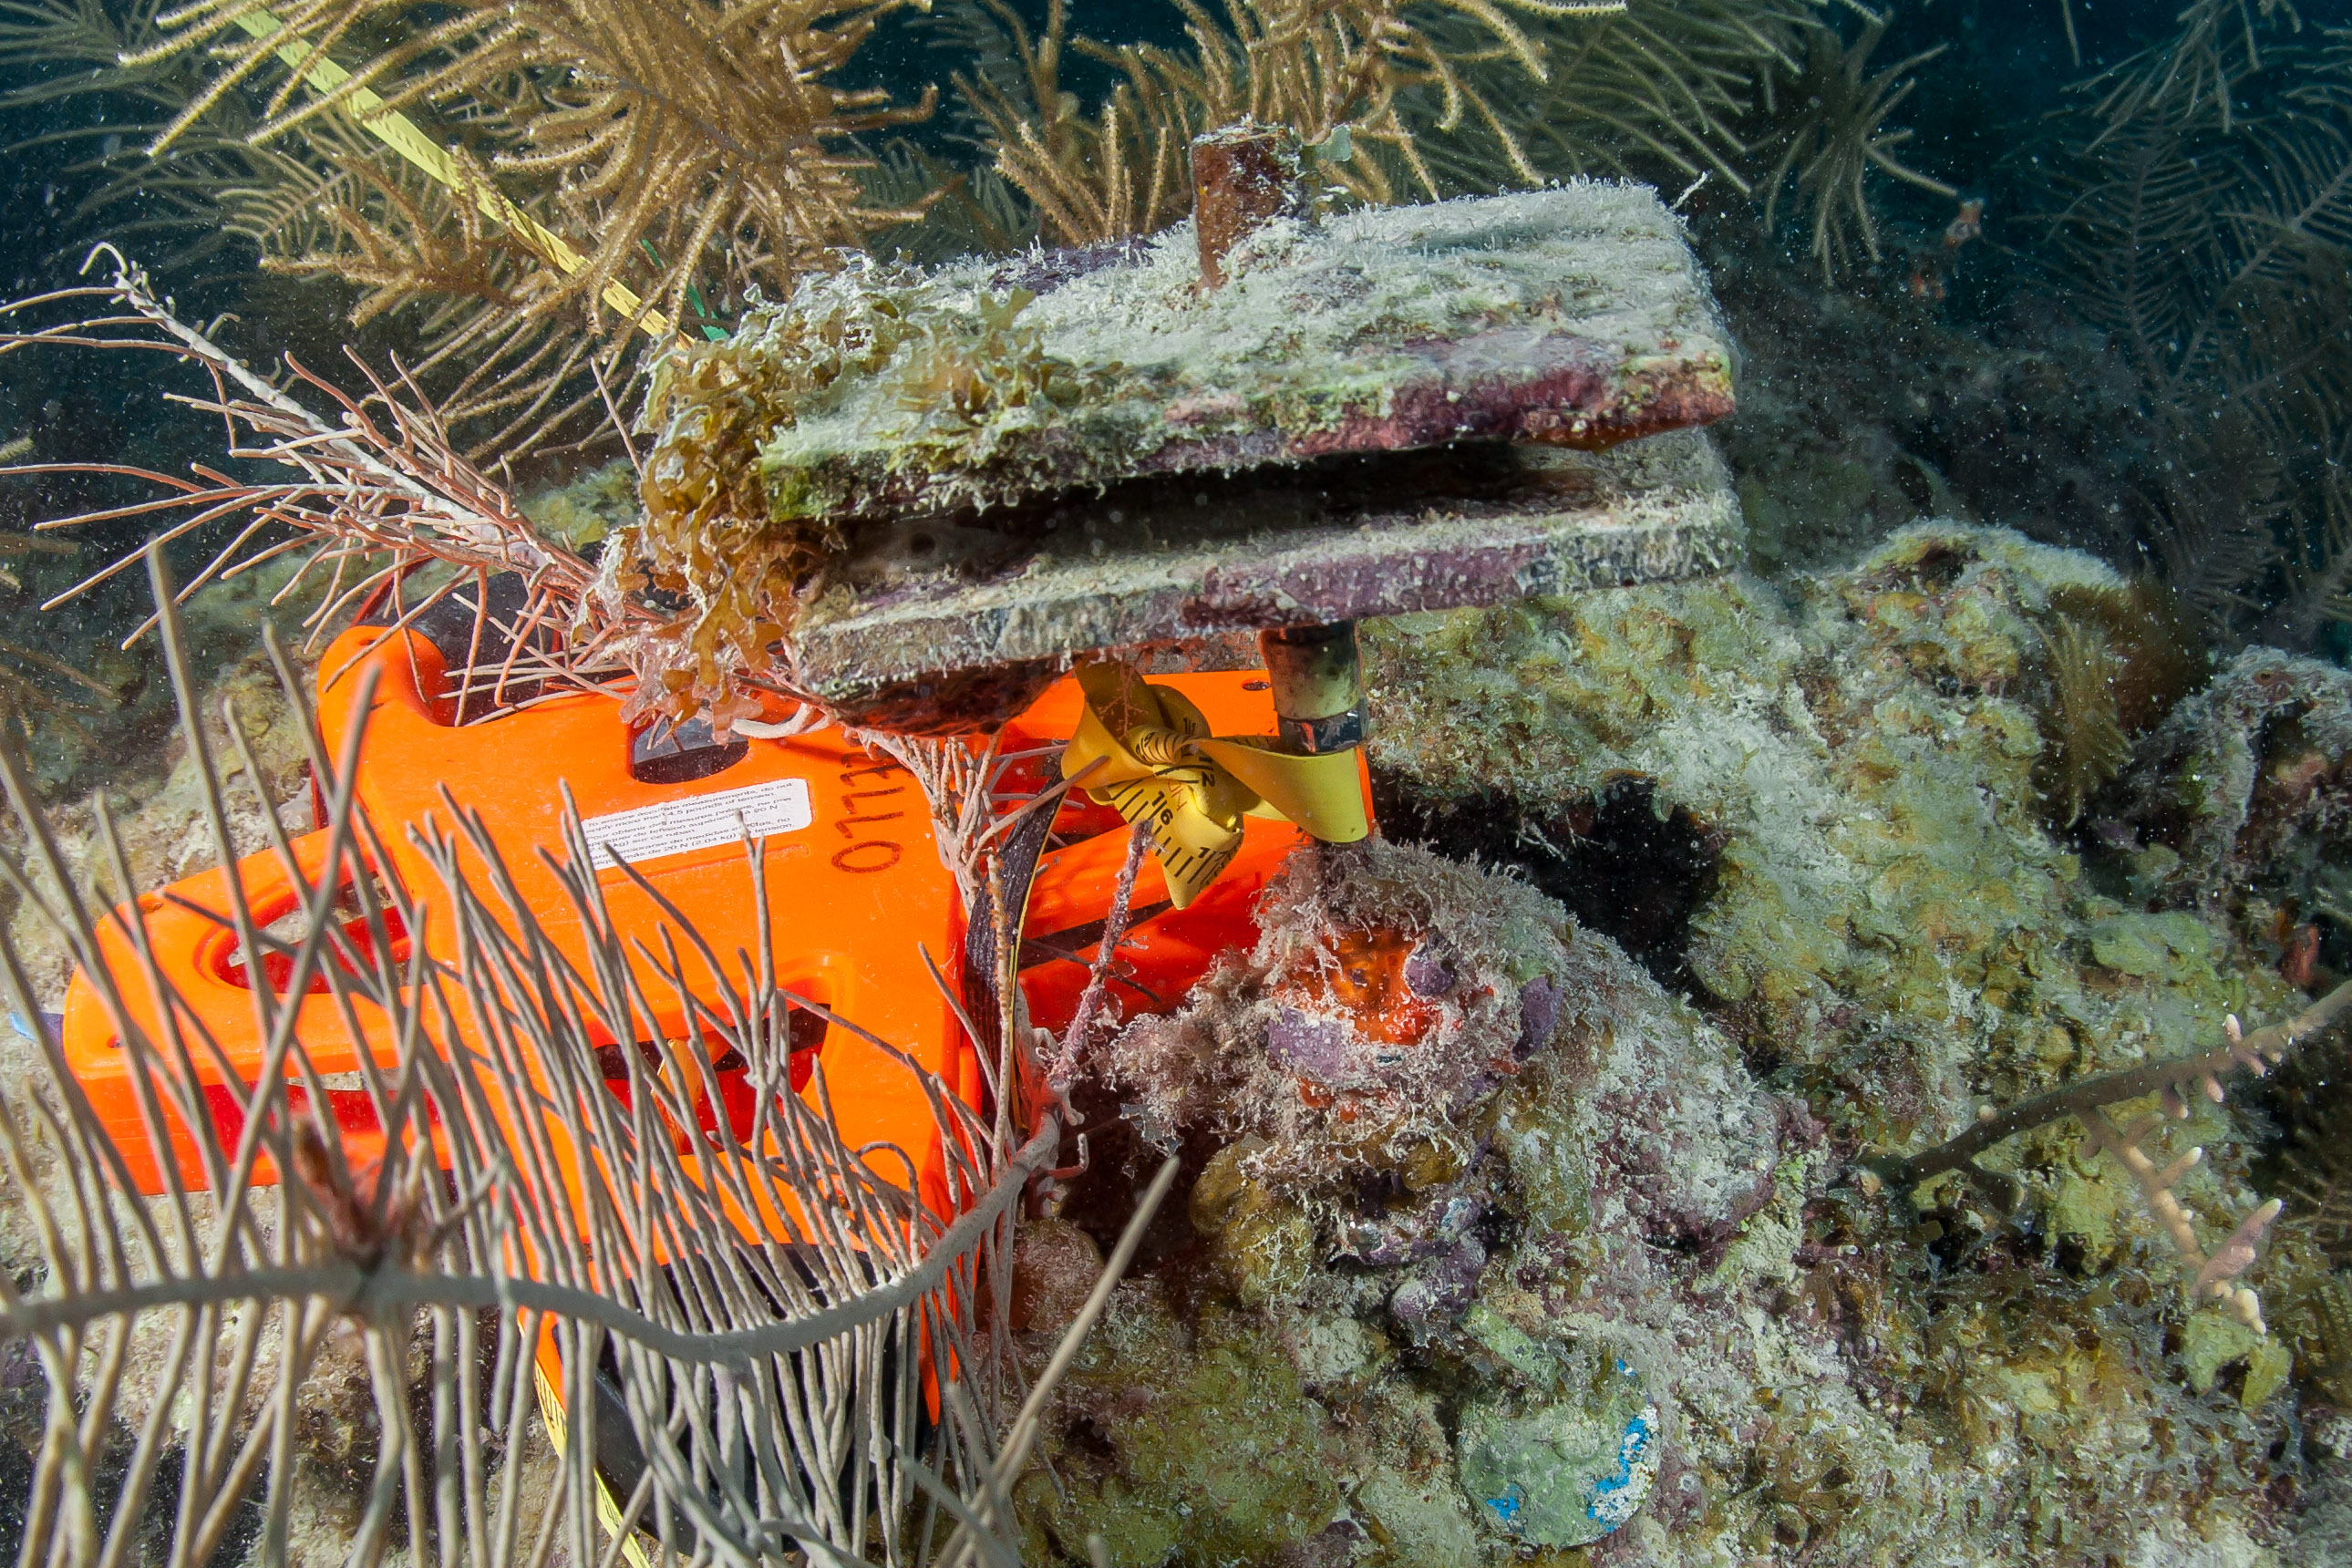
\includegraphics[width=0.5\linewidth]{Data/CAUBMU} 

}

\caption{CAU and BMU pair after being deployed for 3 years}\label{fig:BMUs}
\end{figure}

 \textbf{Figure 4:} CAU and BMU pair after being deployed for 3 years
WHAT IS ON THE TOP AND BOTTOM? DESCROBE THE PICTURE BETTER

\begin{itemize}
\tightlist
\item
  \textbf{Landscape mosaics} (n=6) and \textbf{carbonate budget} surveys
  (n=6) were completed to monitor changes in benthic cover and carbonate
  production
\end{itemize}

\begin{center}\rule{0.5\linewidth}{0.5pt}\end{center}

\hypertarget{about-the-monitoring-program}{%
\subsubsection{About the monitoring
program}\label{about-the-monitoring-program}}

AOML's climate monitoring is a key part of the National Coral Reef
Monitoring Program of NOAA's Coral Reef Conservation Program (CRCP),
providing integrated, consistent, and comparable data across U.S.
Managed coral reef ecosystems. CRCP monitoring efforts aim to:

\begin{itemize}
\tightlist
\item
  Document the status of reef species of ecological and economic
  importance.
\item
  Track and assess changes in reef communities in response to
  environmental stressors or human activities.
\item
  Evaluate the effectiveness of specific management strategies and
  identify actions for future and adaptive responses.
\end{itemize}

\hypertarget{point-of-contact}{%
\subsubsection{Point of Contact}\label{point-of-contact}}

Atlantic Climate team lead:
\href{mailto:nicole.besemer@noaa.gov}{\nolinkurl{nicole.besemer@noaa.gov}}

Principal Investigator:
\href{mailto:ian.enochs@noaa.gov}{\nolinkurl{ian.enochs@noaa.gov}}

NCRMP Coordinator:
\href{mailto:erica.towle@noaa.gov}{\nolinkurl{erica.towle@noaa.gov}}

\hypertarget{for-more-information}{%
\subsubsection{For more information}\label{for-more-information}}

Coral Reef Conservation Program: \url{http://coralreef.noaa.gov}

NCRMP climate monitoring:
\url{https://www.coris.noaa.gov/monitoring/climate.html}

NOAA Atlantic Oceanographic and Meteorological Laboratory:
\url{http://www.aoml.noaa.gov/}

\href{https://www.coris.noaa.gov/monitoring/status_report/docs/FL_508_compliant.pdf}{Florida
Coral Reef Status Report 2020}

\hypertarget{acknowledgements}{%
\subsubsection{Acknowledgements}\label{acknowledgements}}

These efforts were jointly funded by NOAA's CRCP and OAP. We would like
to thank the National Park Service and Florida Keys National Marine
Sanctuary for permitting support and the ANGARI Foundation for field
support.

\begin{flushleft}\includegraphics[width=0.2\linewidth]{DRTO_Field-Report_AP_V2_files/figure-latex/funding-1} \end{flushleft}

\hypertarget{our-team}{%
\subsubsection{Our Team}\label{our-team}}

\begin{flushleft}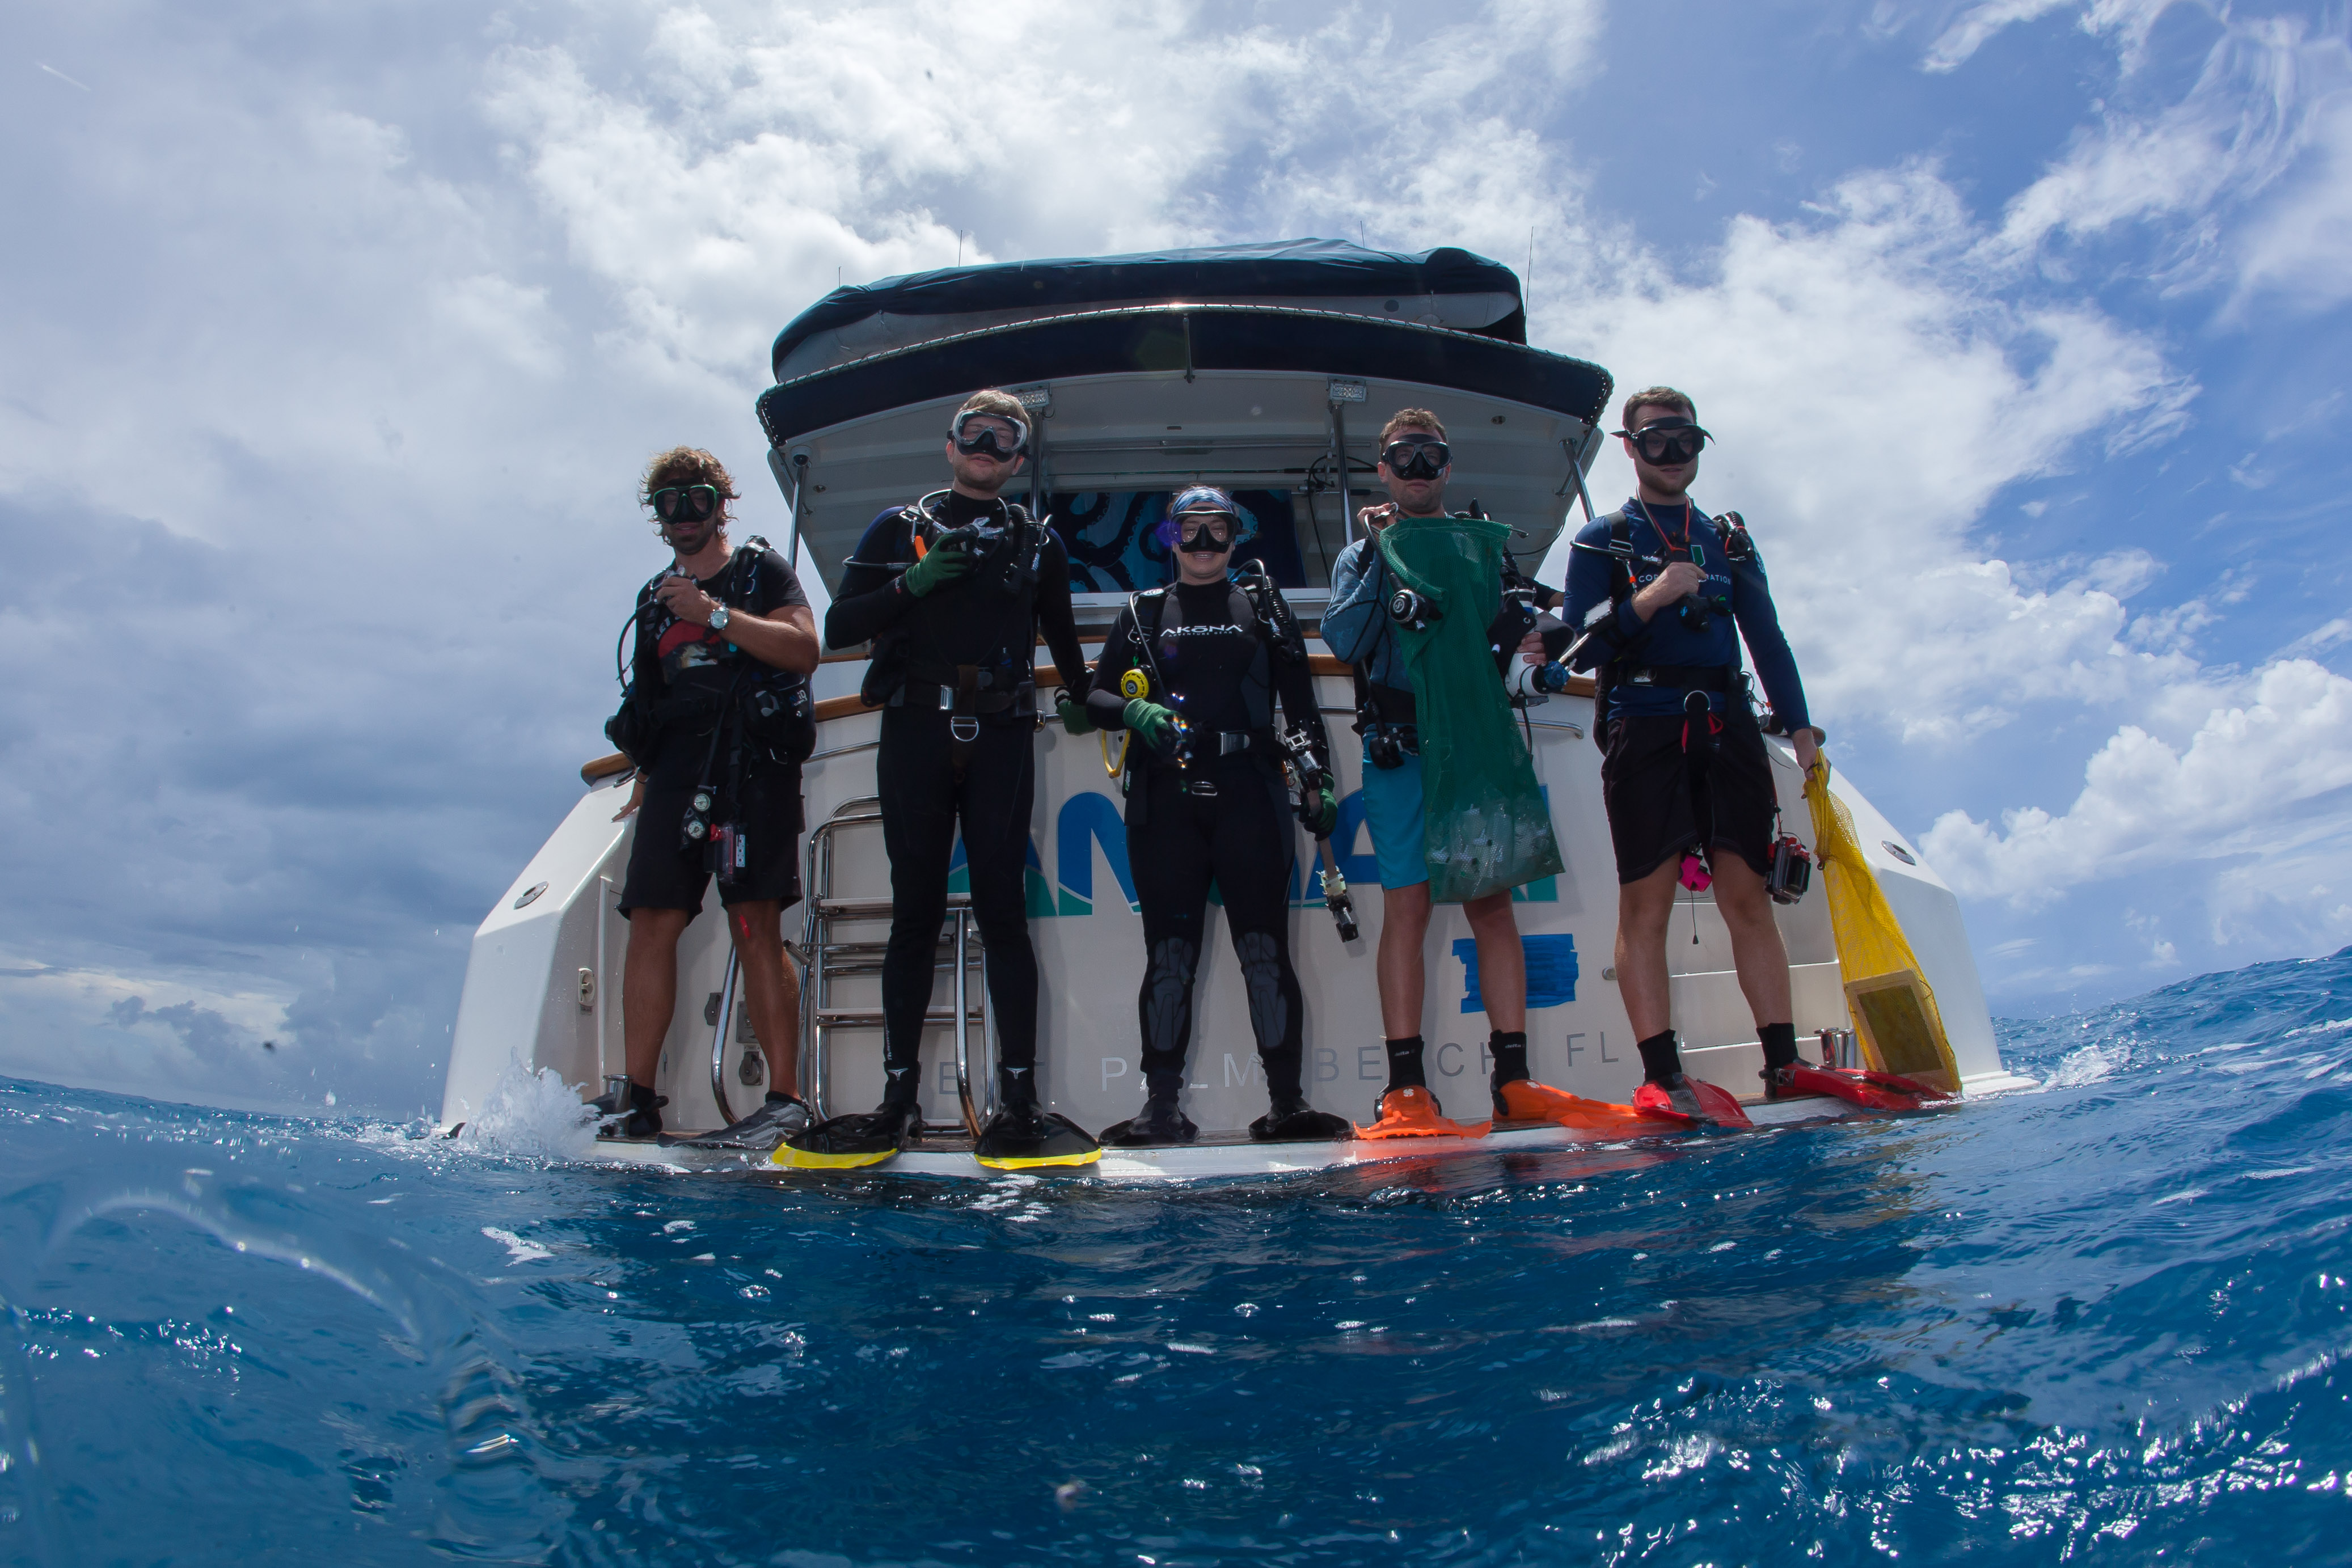
\includegraphics[width=0.5\linewidth]{Data/Fieldteam} \end{flushleft}

\textbf{Field team members}: Anderson Mayfield, Graham Kolodziej, Nicole
Besemer, Nathan Formel, Patrick Kiel

\end{document}
